\documentclass{book}
\usepackage{amsfonts}
\usepackage{amsmath}
\usepackage[gen]{eurosym}
\usepackage[T1]{fontenc}
\usepackage{textcomp}
\usepackage{graphicx}
\usepackage{etoolbox}
\usepackage{titleps}
\usepackage{float}
% use hidelinks to remove boxes around links to be similar to Texinfo TeX
\usepackage[hidelinks]{hyperref}
\usepackage[utf8]{inputenc}

\makeatletter
\newcommand{\GNUTexinfosettitle}{No Title}%

% redefine the \mainmatter command such that it does not clear page
% as if in double page
\renewcommand\mainmatter{\clearpage\@mainmattertrue\pagenumbering{arabic}}
\newenvironment{GNUTexinfopreformatted}{%
  \par\GNUTobeylines\obeyspaces\frenchspacing\parskip=\z@\parindent=\z@}{}
{\catcode`\^^M=13 \gdef\GNUTobeylines{\catcode`\^^M=13 \def^^M{\null\par}}}
\newenvironment{GNUTexinfoindented}{\begin{list}{}{}\item\relax}{\end{list}}


% used for substitutions in commands
\newcommand{\GNUTexinfoplaceholder}[1]{}

\newpagestyle{single}{\sethead[\chaptername{} \thechapter{} \chaptertitle{}][][\thepage]
                              {\chaptername{} \thechapter{} \chaptertitle{}}{}{\thepage}}

\renewcommand{\includegraphics}[1]{\fbox{FIG \detokenize{#1}}}

\makeatother
% set default for @setchapternewpage
\makeatletter
\patchcmd{\chapter}{\if@openright\cleardoublepage\else\clearpage\fi}{\GNUTexinfoplaceholder{setchapternewpage placeholder}\clearpage}{}{}
\makeatother
\pagestyle{single}%


\begin{document}
\label{anchor:Top}%
\chapter{{Chapteùr}}
\label{anchor:Chapt_00eaur}%


value vùr \{No value for `vùr'\}.

In included téxt.

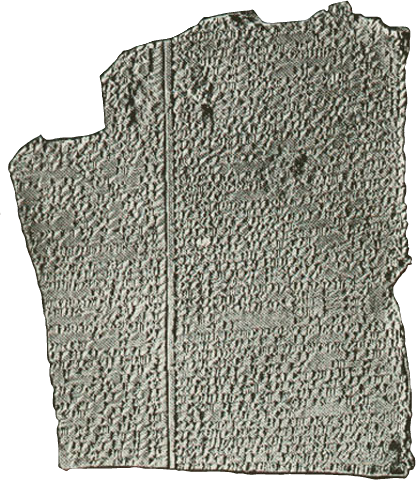
\includegraphics{an_ïmage}
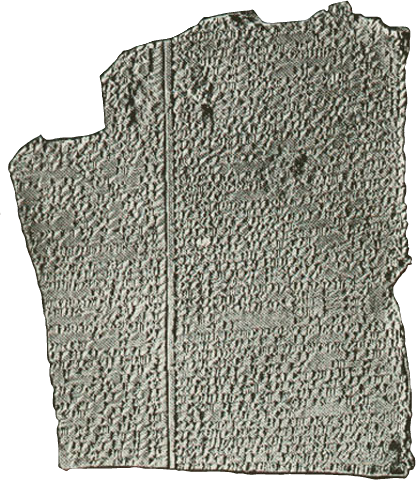
\includegraphics{an_ïmage}

\includegraphics{dîrectory/imàge}


\begin{verbatim}
In included téxt.
\end{verbatim}

\end{document}
